\section{Overview}
The application of mathematics has played a key role in the development of technological advancements and breakthroughs in science. Throughout history, mathematics has provided us with an increasing number of various sub-branches such as discrete mathematics, applied mathematics, cartesian geometry, algebra, calculus and many more. All of which can be applied to the real world, whether it is for construction, physics, or simple day-to-day activities. 

A key branch under discrete mathematics is graph theory where models can be developed to represent relationships between different objects. Graphs contain a range of uses both in the mathematical world and the real world. They can be used to visually represent large sets of numerical data providing a way to deduce different properties and the correlations they have within the data. Examples include identifying clustering of certain areas, the connectivity between vertices or edges and many others. Graphs are also widely known as networks with some examples such as a friendship network, business networks and even food chain levels. Graph theory is the area that I will explore along with a method to visualise them through the help of using python. As well as analysing specific properties that may influence the visualisation of the graphs and thus the outcome of any key relationships between the vertices.

\section{History}
Initially, graph theory was introduced in 1735 as a form of a solution to the seven bridges of Königsberg problem which was solved by Leonard Euler \cite{POWELL20151}. This famous problem involved an island within Königsberg that had a river, Pregel, surrounding the island via a fork. There were seven bridges that crossed the river Pregel from the island to connect to other major landmasses of Königsberg, Prussia. The island had four bridges, two north, two south connecting the mainland and the island. Also another bridge connecting to a neighbouring island and this neighbouring island itself had two bridges. Consequently, giving a total number of seven bridges as stated by the seven bridges of Königsberg problem, see Figure \ref{fig:Königsberg's Bridges} sourced from MacTutor Archive \cite{MacTutor}. 

Due to the location in which the island was situated, the problem was to determine whether a route exists that manoeuvres through all the bridges exactly once and must return to the starting location. Leonard Euler proceeded to analyse the problem by evaluating only the key areas, this was the land masses and the bridges. Other information such as the sizes of the island, bridge type or length were irrelevant. Consequently, the problem could be portrayed by utilising dots and lines \cite{pryor2011seven} to give a simplistic view (see Figure \ref{fig:Königsberg's Graph}). Once developed, the dots are known as vertices which represent the key interests and the edges that are incident to these vertices represent the connections/relationships between them.

By removing the irrelevant information, Euler was able to simplify and visualise the problem. In doing so, Euler discovered the fact that for a solution to exist, each vertex must have an even number of edges incident to them (even degree). This is because you require one edge for entering and another for exiting. Otherwise not all edges will be included in the final path that is based on the conditions of the bridge problem. All vertices in the Königsberg problem have odd degree, meaning that a \emph{Eulerian path} (path that traverses all edges exactly once) does not exist for this problem. Since a Eulerian path does not exist then a \emph{Eulerian circuit} (Eulerian path that returns to the starting vertex) cannot exist either. Therefore, Euler proved that there were no solutions to the seven bridges of Königsberg problem. This proof is regarded as the first proof in relation to graphs and led to the birth of graph theory.

\begin{figure}[!htb]
\centering
\begin{subfigure}{.45\textwidth}
	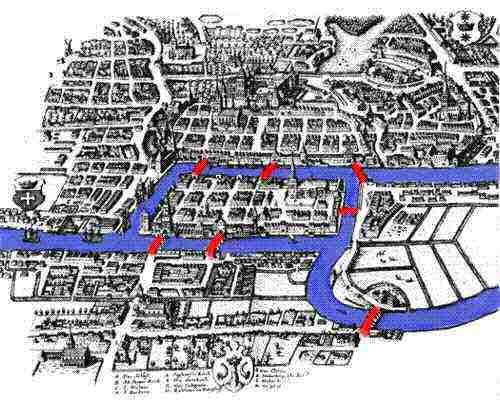
\includegraphics[scale=0.4]{Konigsberg}
	\caption{}
	\label{fig:Königsberg's Bridges}
\end{subfigure}
\hfill
\begin{subfigure}{.45\textwidth}
	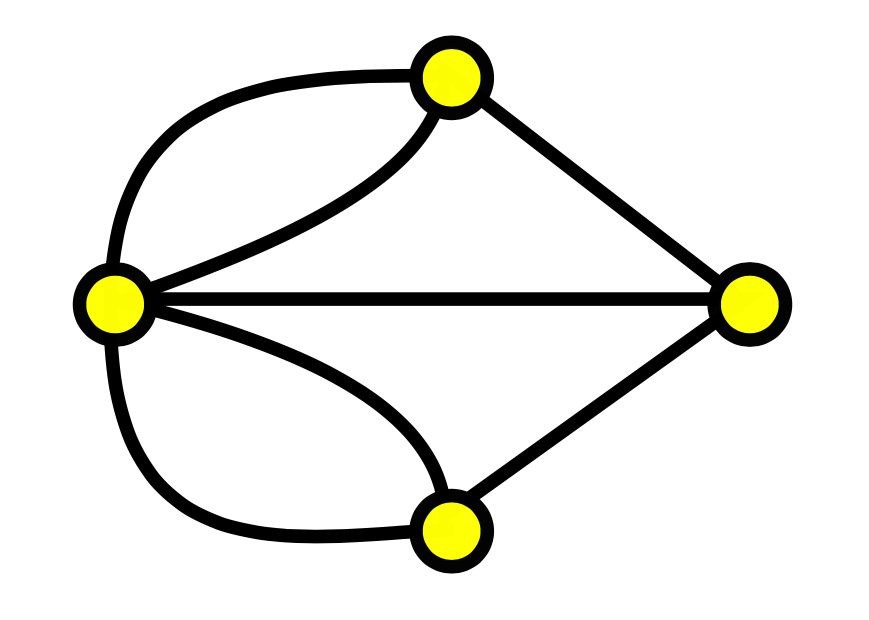
\includegraphics[scale=0.45]{Konigsgraph}
	\caption{}
	\label{fig:Königsberg's Graph}
\end{subfigure}
\caption{The (a) original seven bridges of Königsberg and its (b) graph representation that only focusses on the key details and disregards irrelevant information. Achieved by using vertices and edges.}
\end{figure}

Eulerian paths and cycles were a major milestone in the study of graph theory. Based on their unique definitions, they have been a useful tool in graph theory and other scientific fields. An example is the study of DNA fragment assembly through the identification of Eulerian paths. Through these Eulerian paths, repeated DNA fragments can be identified and ``glued" together to construct a \emph{de Brujin} graph. A de Brujin graph is a directed graph that represents overlaps between sequences or symbols. In DNA sequence assembly, traversing a de Brujin graph with overlapping regions can give the full genome sequence. This is studied extensively seen in the paper by Pevzner, Tang and Waterman \cite{pevzner2001eulerian}.

After Eulerian paths and cycles \cite {victor2010eulerian} were introduced, the next famous puzzle in relation to graph theory was invented in 1857 and was known as the Icosian Game \cite{carlson_2022} by William Rowan Hamilton. The objective of the puzzle was to find a cycle that visits all vertices exactly once and returns to the starting vertex. This type of cycle is later defined as a \emph{Hamilton cycle} \cite{rahman2005hamiltonian} along with the definition of a \emph{Hamilton path} which does not have the requirement to return to the starting vertex.

In the mathematical world, Leonard Euler is known for \emph{Euler's identity} in complex mathematics which states that for a real number $x$, $e^{ix}=\cos(x)+i\sin(x)$. This has been crucial in many subject areas such as physics and engineering. Additionally in 1850, Euler uncovered another formula to be known as \emph{Euler's polyhedra formula} which states that $F + V - E = 2$ where $F$ denotes the number of faces, $V$ as the number of vertices and $E$ as the number of edges for a graph model. As polyhedrons can be depicted as graphs, algebraic topology benefited from Euler's polyhedron formula where more complex surfaces could be studied such as the surface of a torus. Based upon this formula, the \emph{Euler characteristic} was formalised to describe the topological characteristic of various complex surfaces with its formula as $F + V - E = 2 - 2g$ where $g$ is denotes the number of ``holes" the surface has (formally known as the \emph{genus}). 

Furthermore, graph theory has assisted in problems such as the four-colour map problem which was introduced in the 1850s. The problem is if all the countries in the world can be coloured with only the use of four colours such that no two adjacent countries were coloured with the same colour. In which the solution was not found until 1972 by Kenneth Appel and Wolfgang Haken \cite{Ohnishi2009} through the assistance of a computer. An alternative example of a four colour problem is the colouring of the counties in the UK with only four colours where the solution for this is shown in Figure \ref{fig:UK 4 colour} sourced from Robin Wilson \cite{4ColourRobin}.

\begin{figure}[!htb]
\centering
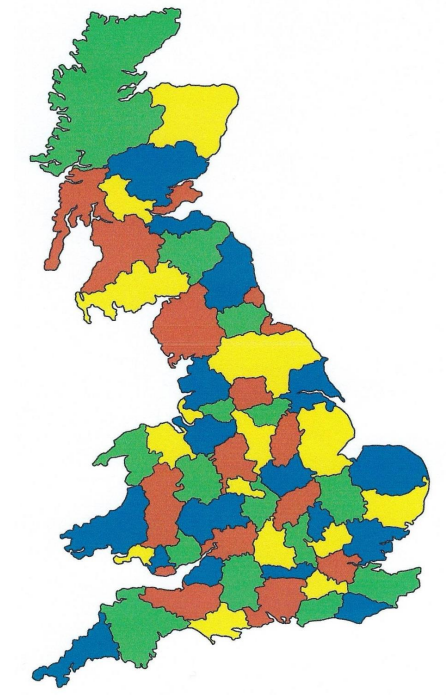
\includegraphics[scale=0.5]{4colourUK}
\caption{The solution for the four colour map problem with regards to the counties in the UK.}
\label{fig:UK 4 colour}
\end{figure}

The Chinese postman problem is another such graph theory problem where you must find the shortest path that uses all the edges in the graph at least once. A similar alternative version is called the travelling salesman problem. In which you identify a shortest path that uses all edges exactly once in the graph and must end at the starting vertex. These such problems are used in Linear programming to find optimal solution in routing or pathing between locations. Variants of the CPP (Chinese postman problem) includes undirected Chinese postman problem (UCPP) and contains different restrictions depending on the subset of edges used (see the paper \cite{IrnichStefan2008Uppw}). Also there exists the Chinese postman problem with load-dependent costs (CPP-LC \cite{CorberánÁngel2018TCPP}) that includes weights on the edges so that an optimal route can be generated. This can widely be used and applied to problems such as the best route to lower a vehicle's CO$_2$ emission. These problems can be applied to modern day scenarios which means that they are still valuable to companies now.
\newline

Therefore, studies within graph theory have been researched extensively since 1735 with many beneficial factors brought into the real world. This is possible due to the versatile nature that data structures in the real world can be represented as mathematical structures through graphs or networks. Examples of what they can represent ranges from simple relationships between people to the complex structure of the brain by studying the brain's anatomic structure and assigning vertices according to the sections of the brains and edges as the links between them. The links are typically representations of the neurons in the brain. Further details of brain mapping into graphs can be read by the paper \cite{articlebrain}. Therefore, by using graph models, various patterns and correlations can then be derived to generate graph properties. These properties can be studied to develop useful information and possible improvements to the whole graph.

\section{Basic notation and terminology}
Graphs or networks are mathematical constructs that are formed by a collection of vertices and edges. Vertices $V$ represents individual objects such as land masses, companies, houses, people, etc. Edges $E$ represents the connections between the vertices such as their relationship, flow of water, supply chain, etc. Sets $V(G)$ or $V$ and $E(G)$ or $E$ forms the graph $G$ and can be written as $G=(V, E)$ with E being a subset of $V \times V$. So an edge $e \in E$ can be written as $v_{1}v_{2}$ if $e$ connects $v_{1}$ and $v_{2}$ where $v_{1}, v_{2} \in V$. There exist variations among graphs as they can be directed or undirected, the edges may carry weights and they may contain self-loops. Figures \ref{fig:Simple Graph} and \ref{fig:Directed Graph} show simple graphs, one of which is undirected, and another is directed. A graph $H = (V', E')$ is a \emph{subgraph} of $G=(V, E)$ if $V' \subset V$ and $E' \subset E$.

\emph{Order} is the mathematical term that represents the number of the vertices in the vertex set $V(G)$. \emph{Size} is number of edges or vertex pairs in the edge set $E(G)$. The \emph{degree} of a vertex, denoted by $deg(v)$ is the number of edges that are connected (otherwise known as \emph{incident}) to the vertex, discussed previously in Euler's solution to the seven bridges of Königsberg problem. Additionally, $\delta(G)$ and $\Delta(G)$ represents the \emph{minimum} and \emph{maximum degree} in $G$ respectively. $G$ is a \emph{regular} graph if $\delta(G) = \Delta(G)$. Vertices $v_{1}$ and $v_{2}$ are \emph{adjacent} if there exists an edge $e \in E$ that connects them. Vertex $v_{2}$ is also known as a \emph{neighbour} to $v_{1}$ and is part of the set $N(v_{1})$ which denotes the neighbours of $v_{1}$. 
\newline

\begin{figure}[!htb]
\centering
\begin{subfigure}{.45\textwidth}
	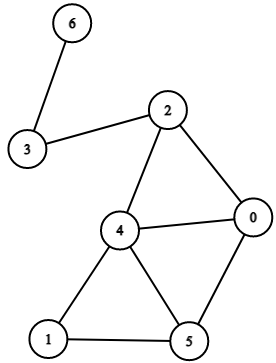
\includegraphics[scale=0.9]{simplegraph}
	\caption{An undirected graph with 7 vertices, 9 edges and an average vertex degree of $18/7$.}
	\label{fig:Simple Graph}
\end{subfigure}
\hfill
\begin{subfigure}{.45\textwidth}
	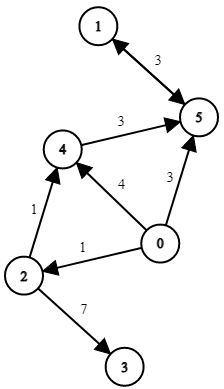
\includegraphics[scale=0.9]{directedgraph}
	\caption{A directed graph with 7 vertices and 7 directed edges that contain weighted edges.}
	\label{fig:Directed Graph}
\end{subfigure}
\caption{The two simple types of graphs within graph theory that are the basic building blocks for more complex structures and theorems.}
\end{figure}

There are multiple ways to traverse a graph \cite{rahman2017basic}. A \emph{walk} $w = v_1v_2v_3v_4v_5...v_n$ is a sequence of vertices such that $E(w) = (v_1v_2,...,v_{n-1}v_n)$ where vertices and edges can be revisited. They can be \emph{open} or \emph{closed} depending on whether the final vertex is equal to the starting vertex, open if equal and closed if not. A \emph{trail} is an open walk where no edges are revisited but vertices may be revisited. When all the edges are traversed exactly once, it is known as a \emph{Eulerian trail} (mentioned previously as a Eulerian path) and the graph is called \emph{semi-eulerian} or \emph{traversable}. Similarly for a trail that is closed (returns to the start), then it is known as a \emph{circuit} and if all edges are used then it is called a \emph{Eulerian circuit} (or Eulerian cycle) and the graph is defined to be \emph{Eulerian}. A \emph{path} is a trail but with no vertex repetitions and if the size of the path is equal to the size of the graph, then it is a \emph{Hamilton path}. Finally, a \emph{cycle} is a path that ends at the starting vertex and if all vertices are visited exactly once, then it is known as a \emph{Hamilton cycle} meaning that the graph is \emph{Hamiltonian}.
\newline

When considering network with flows \cite{ford1956network}, vertices can be known as nodes and may have capacities that limit the overall flow through the network shown in Figure \ref{fig:Network Flow}. These networks are especially used when considering plumbing, water pipes and even evacuation routes in a building. Within a room there is a capacity that is represented by the node's capacity and the weights of the edges can demonstrate the rate of flow along with its maximal flow. In other words, when people are evacuating a building, the corridors have a limit to the amount of people that may pass through. Networks can be used to model social network processes through the study of small corporate groups to generate a communications network. This network representation will have a flow of sentiments based on social network theory \cite{ZACHARY1984259} that is constrained in three ways. Firstly, by any existing direct relationships within the group, that will be denoted by vertices. Secondly, the frequency of communication of the relationships defined in the first point. Lastly, the breadth of the existing relationships in the network. Thus, by using graphs and networks, social behaviours within groups or companies can be studied giving ways to more phycological information represented by numerical data.

\begin{figure}[!htb]
\centering
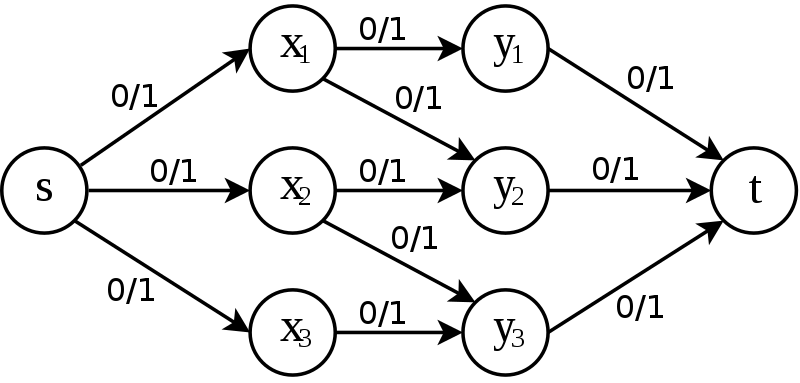
\includegraphics[scale=0.65]{networkflow}
\caption{A simple network flow with a source node and a sink node, the current flow is 3 and the edge capacities are shown.}
\label{fig:Network Flow}
\end{figure}

Additionally, graphs can be represented by using matrices to enable the use of matrix calculations on the datasets. These matrices are known as \emph{adjacency matrices} \cite{KnauerU.2011Agt:} and this matrix contains the number of edges incident to each vertex. The connections of the vertices are based on the location of this value as the rows and columns represent the vertices. A \emph{weighted adjacency matrix} will instead hold the weights of each edge in the matrix. An $n \times n$ adjacency matrix $A = (a_{ij})$ for $ i, j = 1, ..., n$ is defined by $a_{ij} = 1$ if there exists an edge from vertex $i$ to vertex $j$. A matrix is always symmetric when considering an undirected simple graph as an edge will contribute to both sides of the matrix. Examples of an adjacency matrix along with its graph representation is shown in Figure \ref{fig:Adjacency Graph}.
\newline

\begin{figure}[!htb]
\centering
$\vcenter{\hbox{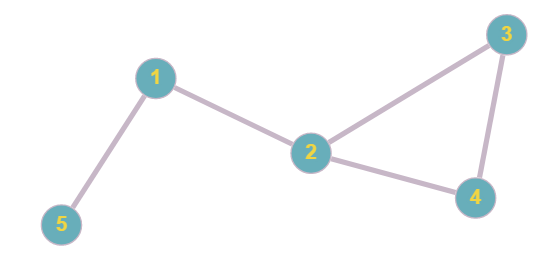
\includegraphics[scale=0.6]{adjgraph}}}$
\hfill
$A = \begin{pmatrix}
0 & 1 & 0 & 0 & 1 \\
1 & 0 & 1 & 1 & 0 \\
0 & 1 & 0 & 1 & 0 \\
0 & 1 & 1 & 0 & 0 \\
1 & 0 & 0 & 0 & 0 \\
\end{pmatrix} $
\caption{A simple graph along with its adjacency matrix.}
\label{fig:Adjacency Graph}
\end{figure}

\section{Linguistic and Lexical Analysis}
Both the linguistic and lexical field can use the implementation of graphs to further generate relations between words or characters based on a given text \cite{vitevitch2008can}. Vertices would represent each word or character and the directed edges would be the connections in relation to their text. A simple word graph example is seen in Figure \ref{fig:diddle} created from the poem ``Hey Diddle Diddle" by Walter Crane \cite{crane2016baby}. Instead of directed graphs, trees can be used as an alternative to display the same text. However, for clarity, we only look at directed graph representation. 

\begin{figure}[!htb]
\centering
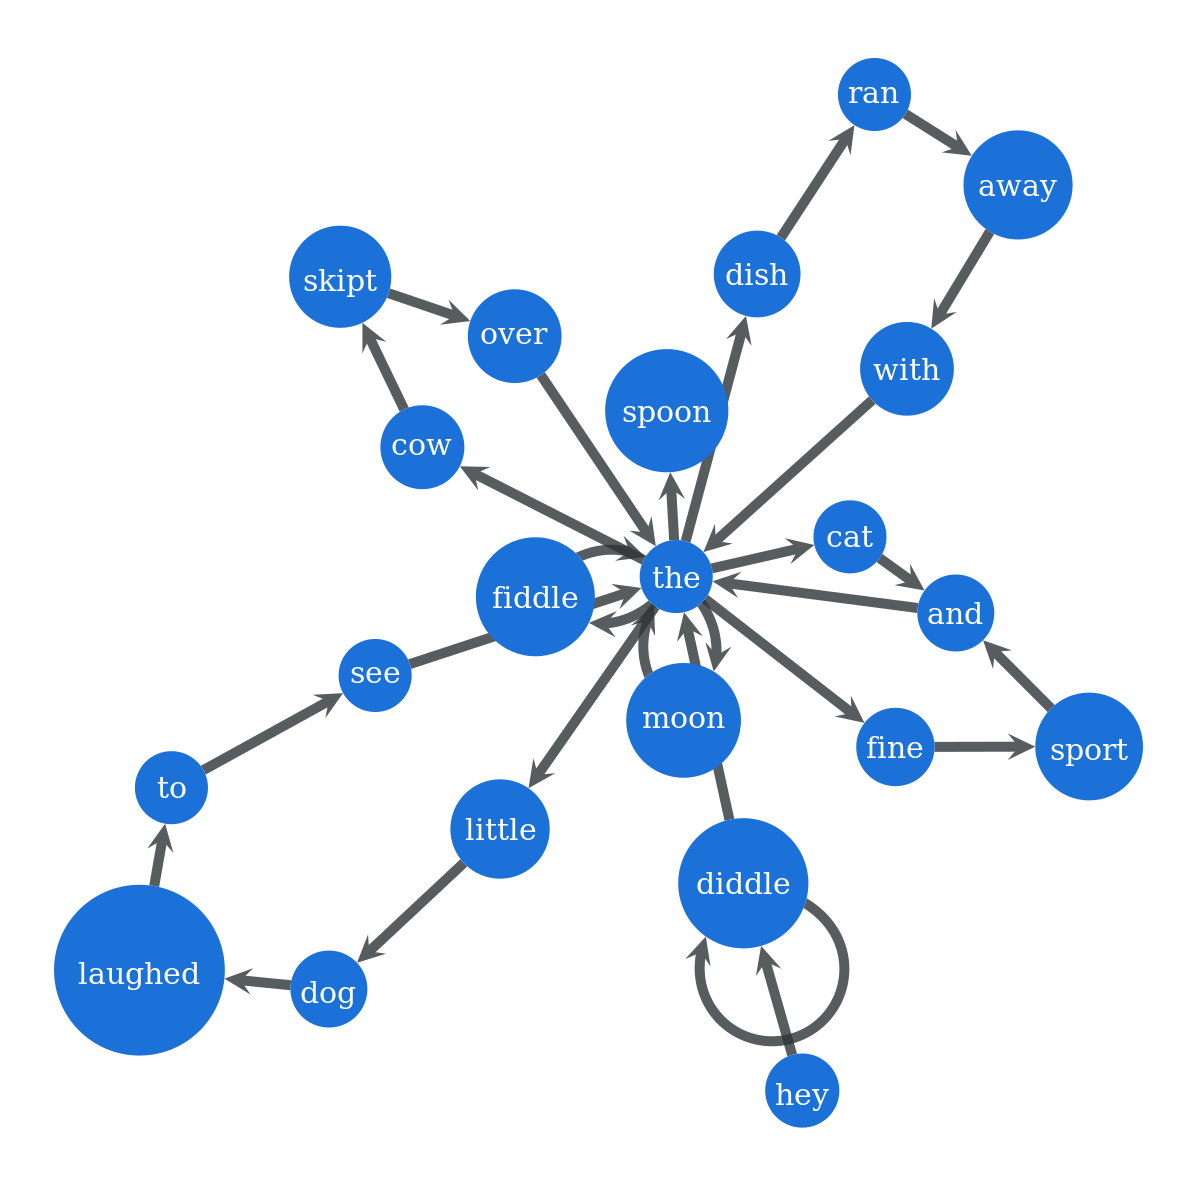
\includegraphics[scale=0.25]{diddle}
\caption{Directed word graph for the poem ``Hey Diddle Diddle" by Walter Crane.}
\label{fig:diddle}
\end{figure}

Correlations can be identified through the study of word graphs, and they can exhibit unique characteristics such as the small-world characteristic. The small-world characteristic is based on the combination of high clustering and short path lengths where it is observed that a high degree of local clustering also has efficient global connectivity (short path lengths to other vertices). Clustering will be explored in detail in the next chapter. This small-world characteristic is often described as the ``six degrees of separation" and more can be read in the paper by Watts and Strogatz \cite{watts1998collective}. 

In any natural language, words are essential building blocks to formulate expressions and meaning when conversing or writing. They can become complex because words may have various meanings and tenses such as the past, present, and future tense in the English language. Linguistic analysis is the study of natural language texts such as English, its grammar and the structure. Lexical analysis is similar but instead of studying words, it is the study of tokens or characters. For example, lexical analysis can be on the variants of the same word given their tense \cite{hippisley2010lexical}. Whereas linguistic analysis determines the importance of words in a text and their relative positioning in its structure. Additionally, their syntactic and semantic information \cite{broekman2021linguistic}. Essentially Lexical analysis is a branch of linguistic analysis. The goal of my research is the study of languages with various graph representations, to study properties of relationships between words in each text. Therefore, we are mainly focussed on linguistic analysis rather than lexical analysis.

The focus for future chapters will be on directed graphs and the data that can be extracted from them. Chapter 2 will describe and outline specific complex graph properties that will be applied to datasets later. This means that by analysing the graphs, numerical values can be generated to represent certain factors of the graph. These factors can then be applied to the graph to rearrange its shape so that further correlation can be identified between all the vertices and edges. We will explore linguistic analysis and study datasets generated based on different languages. But to achieve this, we will first discuss the graph properties that could assist in identifying correlations before the language datasets.